\documentclass{article}
\usepackage{graphicx} % Required for inserting images
\usepackage{amsmath}

\def\apj{ApJ}
\def\apjl{ApJ Lett.}
\def\mnras{MNRAS}
\def\nat{Nature}
\def\physrevB{Phys. Rev. B}
\def\prd{Phys. Rev. D}
\def\prl{Phys. Rev. Lett.}
\def\pre{Phys. Rev. E}
\def\araa{Ann. Rev. Astron. Astrophys.}                % "Ann. Rev. Astron. Astrophys."
\def\aap{Astron. Astrophys.}                  % "Astron. Astrophys."
\def\aaps{Astron. Astrophys. Suppl. Ser.}                 % "Astron. Astrophys. Suppl. Ser."
\def\aj{Astron. J.}                      % "Astron. J."
\def\apjs{Astrophys. J. Suppl. Ser.}                  % "Astrophys. J. Suppl. Ser."
\def\pasp{Publ. Astron. Soc. Pac.}                  % "Publ. Astron. Soc. Pac."
\def\apjl{ApJ Lett.}                   % letter at ApJ
\def\pasj{PASJ}
\def\apss{Astroph. Space Sci.}
\def\aplett{Astroph. Lett.}
\def\ssr{Space Sci. Rev.}
\def\jcap{J. Cosmol. Astropart. Phys.}
\def\apspr{Sov. Sci. Rev. Sect. E}
\def\nar{New Astron. Rev.}
\def\aapr{ Astron. Astrophys. Rev.}

\title{fbotCompton}


\begin{document}
	
	\section{Introduction}
	Fast Blue Optical Tranients are highly luminous objects with very fast rise and decay 
	phases discovered in optical  
	Recent observations of Fast Blue Optical Transients 
	%koala has not X-ray
	\cite{Margutti2019, Ho2019cow,Ho2020koala,Coppejans2020, Ho2021at2020, YaoAt2020mrf, MatthewsAT2022tsd, CHrimesAT2023fhn},  show high level of X-ray radiation. There are suggested different scenarios of  origins of this radiation: central engine or interaction of shock with external medium. In this paper we present model of interaction of shock with strong wind from close star, producing X-ray emission via inverse Compton scattering on the photons of this star. This assumption is supported by studying of local environment of object AT2018cow \cite{SunAT2018environment} showing that there are two young massive star clusters in vicinity of AT2018cow. Young massive star clusters (YMSC) have a lot of stars with strong winds and high luminosity in rather small volume (f. e. cluster Westerlund-1 has 6 yellow giants, 4 red supergiants, 24 Wolf-Rayet stars, and dozens of OB stars in the radius of 1 parsec \cite{Clark2005westerlund, Crowther2006westerlund, Negueruela2010westerlund}). So if supernova explosion happens in YMSC, it is probable that ejecta will interact with strong wind of neighbour star, placed at distance about $10^{17}~cm$.  In this work we use object CSS161010, described in \cite{Coppejans2020}, because it has very high ejecta velocity ($0.3 c - 0.5 c$) and it makes Particle-in-Cell (PIC) modeling of particle acceleration, which we use to obtain distribution function of emitting electrons, more simple??. This paper is organized as follows: in section \ref{synchrotronChapter} we evaluate synchrotron radio flux from CSS161010 and fit it to observation data, varying such hydrodynamical parameters as magnetic field and number density. In section \ref{hydrodynamic} we present hydrodinamic simulation of interaction between supernova ejecta and stellar wind, using parameters obtained on previous step. And in section \ref{compton} we evaluate Inverse Compton X-ray flux from the region beyond wind bow-shock.
	
	\section{The problem of X-ray}
	While radio emission from CSS161010 can be explained with model of spherical ejecta with self-absorption \cite{Coppejans2020}, as is described in section \ref{synchrotronChapter}, the bright X-ray radiation detected on the 99 day after explosion (flux $F_{X} = (1.33 \pm 0.76)\times10^{-15} erg~s^{-1}~cm^{-2}$ and corresponding isotropic luminosity $L_{X}=(3.4\pm1.9)\times10^{39} erg~s^{-1}$ in range 0.3-10 keV)is not easy to explain.
	At first one can evaluate X-ray part of synchrotron radiation, using parameters provided by authors of \cite{Coppejans2020}. Modeled synchrotron specturm and observational radio and X-ray data (assuming photon index 1.25) are shown on Figure \ref{synchrotronX}. 
	\begin{figure}
		\centering
		\includegraphics[width=0.7\textwidth]{./fig/what.png} 
		\caption{Modeled synchrotron spectrum of CSS161010 and observational radio and X-ray data.}
		\label{synchrotronX}
	\end{figure}
	Also one can assume that electrons spectrum becomes harder on higher energies, it follows from Monte-Carlo simulations \cite{BykovRomansky}. Using obtained in \cite{Coppejans2020} magnetic field $B \approx 0.6~G$ we can calculate the necessary energy of electrons, determined by energy of emitted photon $E_e = (4\pi{m_e}^3 c^5 E_{ph}/0.29\cdot3 e B h)^{1/2} \approx 2\cdot10^6 m_e c^2$. If we assume, that electrons spectrum has index 2 on energies higher than 100 MeV, synchrotron X-ray spectrum would increase. But one should take into account the lifetime of electrons with this energy is $\tau = {m_e}^4 c^7 / e^4 B^2 E_e \approx 10^3~s$ and distance that electron can move on this time is about $d = 3\cdot10^{13}~cm$. This means that emitting volume drastically decreases and we should evaluate radiation of spherical layer with width $d$, and the resulting synchrotron X-ray flux is $what$.
	
	Another option of X-ray radiation is Inverse Compton scattering. The possible seed photons for it may origin from ambient Cosmic Microwave Background and mean galactic field or from the source itself. The ratio of luminocities of synchrotorn and inverse compton radiation of same electrons equals to the ratio of magnetic energy density and photons energy density $L_{IC}/L_{synch}=u_{ph}/u_{B}$. Ratio of radio and X-ray luminocities at 99 day after explosion is $L_{X}/L_{radio} \approx 10$ and the magnetic energy density in CSS161010 is $u_{B}=B^2/8\pi \approx 0.015 erg cm^{-3}$. So to explain X-ray flux as inverse Compton radiation of the same electrons that produce synchrotron radio flux, we need photons energy density about $0.15 erg cm^{-3}$. It is much more than energy density of CMB $4\cdot10^{-13}~erg~cm^{-3}$ and mean galactic photon field $10^{-12}~erg~cm^{-3}$ \cite{Mathis1983} and more than the most luminous stars $L \approx 10^{40}~erg~s^{-1}$ can provide on such distances $L/4\pi R^2 c \approx 10^{-6}~erg~s^{-1}$.
	
	Another distribution of electrons on neighbour star
	
	Estimation of energy
	
	Estimation of synchrotron flux.
	
	\section{Synchrotron radiation}\label{synchrotronChapter}
	Observations of radio flux from CSS16101 \cite{Coppejans2020} shows that it's spectrum is consistent with synchrotron self-absorption model. Method of analytical estimations of source parameters for this case was developed in works \cite{Chevalier1998, ChevalierFransson} and is commonly used to analyze spectrums of FBOTs \cite{Ho2019cow, Ho2020koala, Coppejans2020, Ho2021at2020}. But this approach needs an assumption of power-law distribution of electrons. In this work we use electrons distribution function obtained from PIC simulations of shock wave and evaluate synchrotron radiation using numerical integration of standard formulae for emissivity and absorption coefficient, described in \cite{Ginzburg1975, Ghisellini}.
	
	Distribution function of emitting electrons is evaluated using PIC simulation with code SMILEI \cite{Derouillat}. Setups for shock simulation is described in details in our previous work \cite{BykovUniverse}. Shock was initialized due to collision of uniform plasma flow with velocity $0.3\,c$ with reflecting wall. Magnetization was $\sigma = B^2/4 \pi m_p \gamma c^2 = 0.0002$ and different inclination angles of magnetic field were studied. One can see the well-known effect, that efficiency of particle acceleration strongly depends on the magnetic obliquity to the shock \cite{SironiSpitkovsky2009pair, Crumley2019, GuoSironi2014_1, Romansky2018} on the figure \ref{distributions}, where electron distributions in the shock downstream for different inclination angles are shown.
	
	
	\begin{figure}
		\centering
		\begin{minipage}{0.48\textwidth}
			\centering
			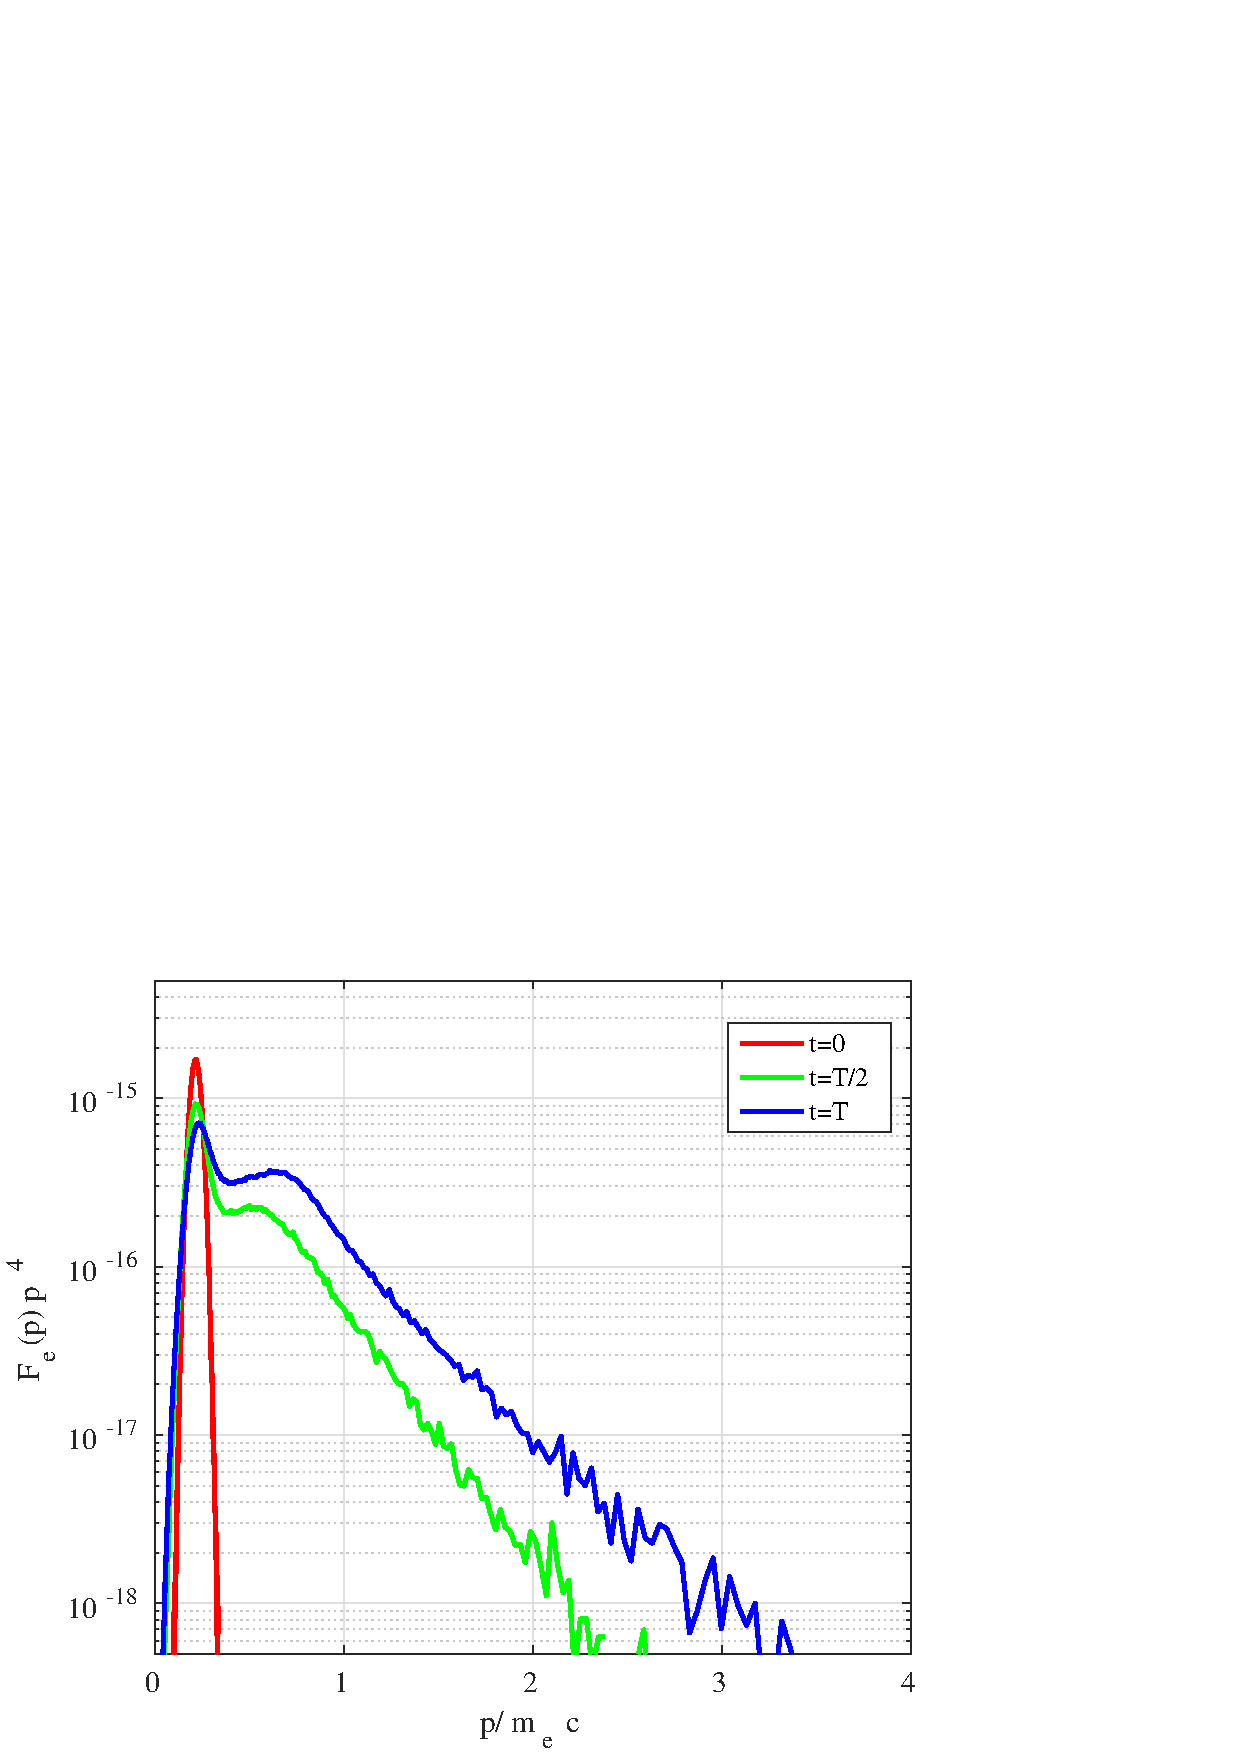
\includegraphics[width=0.98\textwidth]{./fig/electrons.png} 
			\caption{Electron distribution function in the downstream of shock with different inclination angles $\theta$}
			\label{distributions}
		\end{minipage}\hfill
		\begin{minipage}{0.48\textwidth}
			\centering
			\includegraphics[width=0.98\textwidth]{./fig/sphericalSource.png} 
			\caption{Scheme of numerical model of spherical radiation source}
			\label{sphericalSource}
		\end{minipage}
	\end{figure}
	
	For evaluating radiation we use our numerical code FAINA, which allows to evaluate synchrotron and inverse compton radiation and also fit model to observational data. Radiation source in the code is presented as spherical layer in cylindrical coordinates as schematically shown on figure \ref{sphericalSource}. Direction to observer is along z-axis. Colour shows the part of volume of cell is filled with emitting plasma. Each cell has it's own magnetic field, electron number density and distribution. This geometry allows to integrate emissivity along line of sight, taking into account self-absorption. 
	
	Analytical analysis \cite{Coppejans2020} and numerical modeling \cite{BykovUniverse} shows that magnetic field in the system should be rather strong (about $0.3~G$ at distances about $10^{17}~cm$). It does not seems to be possible that quasi-uniform interstellar magnetic field can be so strong. Another option is to use magnetic field generated by the star, but on this distances it should be perpendicular to the shock velocity \cite{Parker} and particle can not be accelerated in quasi-perpendicular shocks, as it was mentioned above. The presence of strong turbulence can increase efficiency of acceleration in quasi-perpendicular shocks, as shown with PIC simulations in works \cite{Demidem2023inhomogenousshock, Bresci2023turbulentchock, Romansky2019turbulence}. But here we use more simple model: PIC simulations are performed with constant initial field, but in evaluation of synchrotron radiation we assume strong largescale turbulence around the star, containing $90 \%$ of magnetic energy, with characteristic scale about radius of expanding ejecta, and Kolmogorov's energy spectrum. Due to fluctuating magnetic field, shock becomes quasi-parallel at some points, and can be a source of accelerated particles. Time of forming the powerlaw tail of electrons distribution in our PIC simulations is much smaller than time of significant changes of magnetic obliquity due the shock movement in this large-scale turbulence, and we consider that electron distribution becomes stationary in every cell of emitting envelope and corresponds to the inclination angle of magnetic field at this point. Number density of electrons is considered uniform inside the radiation source.
	
	We consider radio flux from CSS161010 at 98 day after explosion (the first observation when both radio and X-ray flux was detected). For defining parameters of the source: it's radius $R$, average magnetization $\sigma$, number density $n$, and width fraction of spherical layer $f$, we fitted modeled radiation to observational data and optimized residual, defined as $r(R, \sigma, n, f) = \sum (F(\nu_i, R, \sigma, n, f) - F_{obs}(\nu_i))^2/{\Delta_i}^2$, where summation goes through all observed data points, $\nu_i$ - i-th frequency, $F_obs$ - observed flux, $\Delta$ - uncertainty of observational data. Picture of this residual for fixed parameters $\sigma$ and $n$, and fitted $R$ and $f$ is shown on figure \ref{error}. One can see, that there is long valley of small values of residual and due to systematical uncertanties of our model we cannot peak one point with exact parameters for best fit. Also the global minimum of residual is located in the region of very high magnetization and low density, while shocks can exist only if $\sigma < 1$ \cite{?} and as shown in \cite{Sironi2011magnetization, Lemoine2014} electron acceleration is depressed for magnetization greater than $10^{-2}$. So for further modeling we fix value of $\sigma$ to value $0.0002$, which was used in PIC simulations.
	
	With this assumption, obtained parameters of the source are: radius $R = 1.4\cdot10^{17}$, magnetic field $B = 0.09~G$, number density $n = 2000~{cm}^{-3}$ and shell width $l = 0.12\cdot R = 1.7\cdot10^{15}~cm$. The parameters are broadly consistent with the results of other authors \cite{Coppejans2020}, apart from the electrons number density which is much higher because of quasi-thermal distribution used.  Modeled radio flux and observational data are shown in Figure \ref{synchrotron}. One can see, that peak of the spectral density is provided by thermal electrons, as predicted by \cite{Margalit2021}.
	
	\begin{figure}
		\centering
		\begin{minipage}{0.48\textwidth}
			\centering
			\includegraphics[width=0.98\textwidth]{./fig/error.png} 
			\caption{Profile of residual in plane $\sigma - n$ with other parameters optimized}
			\label{error}
		\end{minipage}\hfill
		\begin{minipage}{0.48\textwidth}
			\centering
			\includegraphics[width=0.98\textwidth]{./fig/radiation2.png} 
			\caption{Observed and modeled radiospectrum of CSS161010 at 98 day after explosion.}
			\label{synchrotron}
		\end{minipage}
	\end{figure}
	
	
	And then we use obtained parameters for hydrodinamical modeling of interaction between sub-relativistic ejecta and strong stellar wind from neighbour star.
	
	
	\section{Hydrodynamic}\label{hydrodynamic}
	In our model we took two close stars, on a distance $1.4\cdot10^{17}~cm$, which corresponds to the radius of expanding shock of CSS161010 at 98 day after explosion. It is  possible in young massive star clusters where are a lot of bright stars with powerful stellar winds (OB, Wolf-Rayet, and red supergiants) in the small volume. We will refer to them as first star - stable, generating wind, and the second - exploded as supernova. We assumed both stars have winds with velocity $v_w = ?$ and mass loss $\dot{M} = 10^{-5} M_\odot $ per year and luminosity $L=500000 L_\odot$ and surface temperature $T = 2.5\cdot10^6~K$ which is typical for Wolf-Rayet stars. The magnetic field of the wind is initialized using \cite{Bjorkman1993}, and for the first star  it's amplitude is $1~G$ at the radius $10~12 cm$ while for the second we need much stronger field to satisfy synchrotron observational data. So we took magnetic field $1000~G$ at the radius $10^{12}~cm$, stars with such strong fields are described in \cite{}.
	
	For hydrodinamcal simulation we use code PLUTO \cite{MignonePluto}. We used several nested setups on different scales. At first we performed 3d modeling of two stable stars with parameters described above until they winds form a stable configuration. First star is placed at point with coordinates $x_1 = 0, y_1 = 0, z_1 = 0$, and the second at point with $x_2 = 0, y_2 = 0, z_2 = 1.4\cdot10^{17}~cm$. Plane x-y is equatorial plane of winds of both stars. Sizes of the simulation box are $Lx = 6\cdot 10^{17}~cm$ and $Ly = Lz = 3\cdot 10^{17}~cm$ with number of grid points 400, 200 and 200 respectively. The next step was 1d spherical modeling of second star explosion. We use ejecta mass $M_{ej} = 0.1 M_\odot$ and velocity $v_{ej} = 0.3\,c$ and initial conditions as described in \cite{ChevalierLiang1989, Petruk2021snr}. The simulation box is split into three regions - in the central region with radius $r_0 = ?$ density is constant and velocity is proportional to radius $v(r) = 0.3 c r/r_0$. In the next region between $r_0$ and $r_1 = 2 r_0$ number density depends on radius as $n(r) \propto r^{-9}$ and velocity is also proportional to radius. And in the last region with $r > r_1$ stellar wind with constant velocity $v_w$ and mass loss $\dot{M}$ is initialized. Profiles of ejecta density at different time moments are shown on figure \ref{snr}.
	\begin{figure}
		\centering
		\includegraphics[width=0.7\textwidth]{./fig/snr.png} 
		\caption{Density profile of supernova explosion.}
		\label{snr}
	\end{figure}
	
	At the third step we simulated setup with smaller scale - with size $Lx = 1.05\cdot 10^{17}~cm$ and $Ly = Lz = 0.9\cdot 10^{16}~cm$ and combined results of the previous steps as initial conditions. Also results of 1d modeling were used as time-dependent boundary condition on the right boundary. And at the last step, in setup with the smallest scale $Lx = 0.3\cdot 10^{17}~cm$ and $Ly = Lz = 1.5\cdot 10^{15}~cm$, which is necessary to resolve bow- and termination shock of the wind of the first star, we use results of the third step as initial and boundary conditions. Number density in different setups and their hierarchy scheme is shown on figure \ref{density}. On the panel a one can see interaction of two winds in large-scale simulation at time before the explosion. On the panel b propagation of ejecta in middle-scale simulation at time $t_1 \approx 1.0\cdot10^7~s$ is shown. On the panel c one can see it in small-scale simulation at time $t_2 \approx 1.1\cdot10^7~s$. Ans on the panel d there is zoomed picture of wind bowshock in small-scale simulation at time $t_3 \approx 1.4\cdot10^7~s$ Magnetic field at the same time moments is shown on figure \ref{Bfield}.
	\begin{figure}
		\centering
		\begin{minipage}{0.49\textwidth}
			\centering
			\includegraphics[width=0.99\textwidth]{./fig/density.png} 
			\caption{Density profile of the system at different time moments}
			\label{density}
		\end{minipage}\hfill
		\begin{minipage}{0.49\textwidth}
			\centering
			\includegraphics[width=0.99\textwidth]{./fig/Bfield.png} 
			\caption{Magnetic field profile of the system at different time moments}
			\label{Bfield}
		\end{minipage}
	\end{figure}
	
	Simulations showed that ejecta of supernovae, moving in interstellar medium has profile with thin and dense peak with number density $n \approx 10^5~cm^{-3}$ and width $d = 10^{16}~cm$, and wide region with number density $\approx 10^4~cm^{-3}$ behind the peak.
	
	The wind bow-shock has radius $R_w \approx 2\times10^{14}~cm$ and number density $n_w \approx 10^9~cm^{-3}$. With this parameters, and luminocity and temperature of the star, one can estimate observed X-ray flux, produced by inverse compton scattering.
	
	\section{Inverse compton radiation}\label{compton}
	
	Let consider different models of origin of X-ray radiation, which observed flux in energy range $0.3 - 10~keV$ is $F_{Xray} (1.33 \pm 0.76) \times 10^{-15}~erg~s^{-1}~cm^{-2}$.
	
	At first, we assume that it is synchrotron radiation from the electron distribution, which is prolonged to much higher energies than it is possible to reach in PIC simulation. 
	
	Another option is inverse compton scattering of accelerated electrons. But there is well-known relation between synchrotron and  inverse compton radiation from same electrons \cite{Ghisellini} - total emitted powers relate to each other as energy densities of magnetic field and photon field. The energy density of magnetic field is $U_B = B^2/8\pi = 0.15 ~erg~cm^{-3}$, and total synchrotron flux is $F_s \approx 10^-16~erg~cm^{-2}~s^{-1}$. So to provide observed X-ray flux about $10^{-15}~erg~s^{-1}~cm^{-2}$ there should be energy density of photon field at least $1~erg~cm^{-3}$ which is much more than energy density of mean galactic photon field $10^{-12}~erg~cm^{-3}$ \cite{Mathis1983} and more than the most luminous stars $L \approx 10^{40}~erg~s^{-1}$ can provide on such distances $L/4\pi R^2 c \approx 10^{-7}~erg~s^{-1}$. If one choose a close distances, photon energy density may be higher, but part of volume of ejecta on this distance would decrease as square of $R$, and there would not be increase in inverse compton luminosity. Also one can consider inverse compton scattering on the self synchrotron radiation. The energy density of synchrotron radiation is easy to estimate via observed synchrotron flux $F_{synch} \approx 10^{-15}~erg~cm^{-2}~s^{-1}$. Synchrotron energy density $U_{synch} = F_{synch}/c \cdot (D/R)^2 \approx 10^{-7}~erg~cm^{-3}$, where $D$ is distance to the source $150~Mpc$, is also too low. So we consider that X-ray radiation is not emitted by the same electrons that produced synchrotron radiation.
	
	In our model X-ray flux is generated via inverse compton scattering in the region of interaction between wind from the first star, and supernova ejecta from the second. Relativistic ejecta has huge bulk pressure and wind is compressed to small region with high number density. Also this region is close to high luminous star, and there are suitable conditions for strong inverse compton radiation. Electrons can be accelerated on the shock fronts or on the shearing flows. So electrons distribution function is ???
	
	We assume that source is a cylinder with radius $R_w$, and height also equals $R_w$, with axis oriented along line of sight, and with uniform number density $n_w = 10^9~cm^{-3}$. 
	and photons distribution corresponds to the radiation of the first star at distance $R_w$. With this parameter modeled X-ray flux in the energy range $0.3-10~keV$ is $F_m = $ which is consistent with observed flux of CSS161010 at 99 day after explosion $F_{obs = }$ \cite{Coppejans2020}.
	
	Also we estimate the synchrotron flux from this source. It should be much smaller than flux from the whole remnant, providing observed synchrotron flux. Once again we estimate it via relation between photons energy density and energy density of magnetic field. Total radio flux is about 10 times smaller than X-ray flux, so if we set limit to fraction of synchrotron flux, emitted from X-ray source as $0.1$ of total radio flux, we can obtain condition on magnetic field of second star ${B_2}^2/8\pi < 0.01 L_2/4\pi c {r_w}^2 \approx 1~G$ at distances about $10^{14}~cm$. It is much smaller than field of the first star, and our hydrodynamical simulation takes it into account/
	
	\section{Conclusions}
	In this work we presented model of origin of luminous X-ray radiation from FBOT CSS61010. 
	
	\ack{
		The~authors  were supported by the RSF grant 21-72-20020. Some of the modeling was performed at the Joint Supercomputer Center JSCC RAS and some---at the Peter the Great Saint-Petersburg Polytechnic University Supercomputing Center.
	}
	\bibliographystyle{iopart-num}
	\bibliography{fbotcompton}
	
\end{document}
